\documentclass[a4paper,12pt]{article}
\usepackage{graphicx}
\usepackage{hyperref}
\usepackage{titlesec}
\usepackage{booktabs}
\usepackage{float}
\usepackage{xcolor}
\usepackage{mathptmx}  % Times New Roman-like font
%\usepackage[backend=biber]{biblatex}
\usepackage{mathptmx}  % Times New Roman-like font
\usepackage{amsmath} 



\title{\textbf{Speech Understanding}\\
\bigskip
\bigskip
\bigskip
{Programming Assignment-1}\\
\bigskip\bigskip\bigskip
{Project Report - Q-2-Task A} 
\bigskip\bigskip\bigskip\\
    {Windowing Techniques and Classifier Performance Using UrbanSound8K Dataset}
}
\bigskip\bigskip\bigskip

\author{\textbf{Prepared By:}\\Om Prakash Solanki (M23CSA521)}

\begin{document}
\maketitle

\newpage
\tableofcontents
\newpage

\newpage
\section{Introduction}
This report presents analysis of the UrbanSound8K dataset, focusing on the implementation of various windowing techniques and their impact on spectrogram generation and classification performance. The dataset, available at https://goo.gl/8hY5ER, contains urban sound excerpts categorized into 10 classes. 

The primary objectives of this task are:
    \begin{itemize}
        \item Implementation and comparison of three windowing techniques: 
        \begin{itemize}
            \item Hann
            \item Hamming
            \item Rectangular windows
        \end{itemize}
        \item Generate spectrograms using the Short-Time Fourier Transform (STFT) for each windowing technique.
        \item Train a simple classifier ( SVM) using features extracted from the spectrograms and evaluate performance.
    \end{itemize}
\newpage
\section{Dataset Description}
The UrbanSound8K dataset consists of 8732 labeled sound excerpts (<= 4s) of urban sounds from 10 classes:
\begin{itemize}
    \item Air Conditioner
    \item Car Horn
    \item Children Playing
    \item Dog Bark
    \item Drilling
    \item Engine Idling
    \item Gun Shot
    \item Jackhammer
    \item Siren
    \item Street Music
\end{itemize}
\newpage
\section{Windowing Techniques}
When analyzing signals, we often need to break them into smaller parts. However, this can cause unwanted distortions called spectral leakage. To reduce this, we use windowing techniques, which shape the signal before processing. 
\subsection{Hann Window}
This window smoothly reduces the signal's intensity at the edges, forming a bell-like curve. It helps in reducing distortions and is commonly used in audio and speech processing.
\subsection{Hamming Window}
Similar to the Hann window, but it does not reduce the signal strength as much at the edges. This makes it useful when we need to balance accuracy and distortion reduction, such as in radar and communication systems.
\subsection{Rectangular Window}
This is the simplest type, where the signal remains unchanged (like a normal cutout). It keeps all the data, but the sudden edges can cause more distortions. It is mainly used when we need all the signal details, despite the leakage.

\newpage
\section{Spectrogram Generation}
A \textbf{spectrogram} is a visual representation of how the frequencies of a signal change over time. It is created using the \textbf{Short-Time Fourier Transform (STFT)}, which breaks a signal into small time segments and applies the \textbf{Fourier Transform} to each segment.
\paragraph{}
Spectrograms were generated using the STFT for each windowing technique. The Python library librosa was used for audio processing and visualization. 
\subsection{Generate a Spectrogram using STFT}
    \begin{enumerate}
        \item \textbf{Divide the signal} into short overlapping windows.
        \item \textbf{Apply a window function} (Hann, Hamming or Rectangular) to each segment.
        \item \textbf{Compute the Fourier Transform} for each segment to get frequency components.
        \item Create a 2D plot:
            \begin{itemize}
                \item \textbf{X-axis (horizontal)} → Time
                \item \textbf{Y-axis (vertical)} → Frequency
                \item \textbf{Color intensity} → Magnitude of frequencies
            \end{itemize}
    \end{enumerate}
    \subsubsection{Fold 1 : Spectrogram}
    \begin{figure}[H]
        \centering
        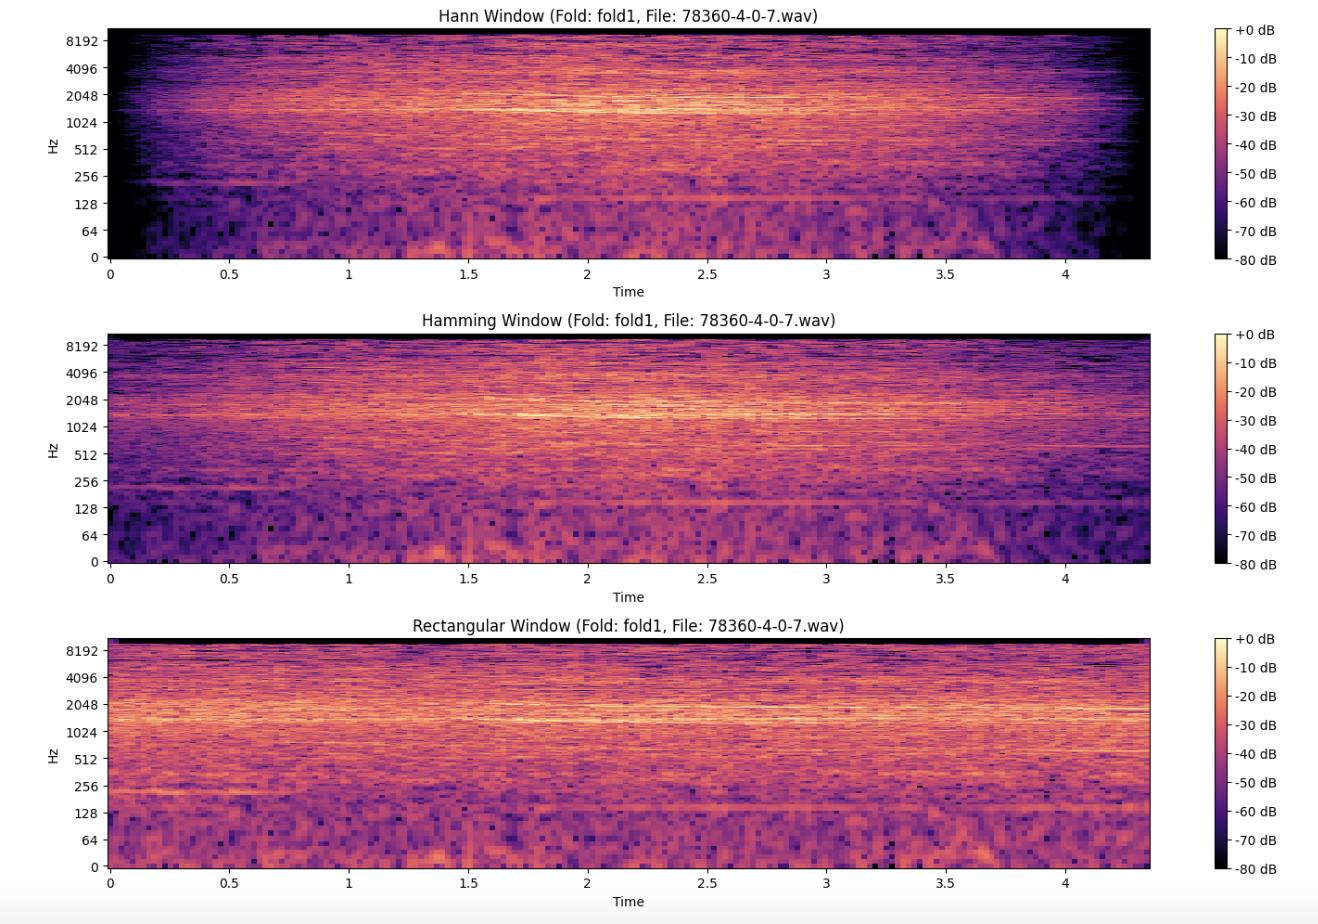
\includegraphics[width=1\linewidth]{Fold1.png}
    \end{figure}
    \begin{itemize}
        \item All spectrograms cover a frequency range from \textbf{0 Hz to 8192 Hz}.
        \item Each spectrogram has a frequency resolution of approximately \textbf{8.28 Hz per pixel}.
        \item The total time duration in all spectrograms is \textbf{4.5 seconds}.
        \item Time resolution is \textbf{0.0033 seconds per pixel}, meaning fine time variations are captured.
        \item \textbf{Hann Window}: Smoother transitions, reduces spectral leakage, slightly lower intensity.
        \item \textbf{Hamming Window}: Similar to Hann but retains more sharpness in mid-frequencies.
        \item \textbf{Rectangular Window}: Higher intensity, but introduces more noise and artifacts.
    \end{itemize}
\newpage
    \subsubsection{Fold 2 : Spectrogram}
    \begin{figure}[H]
        \centering
        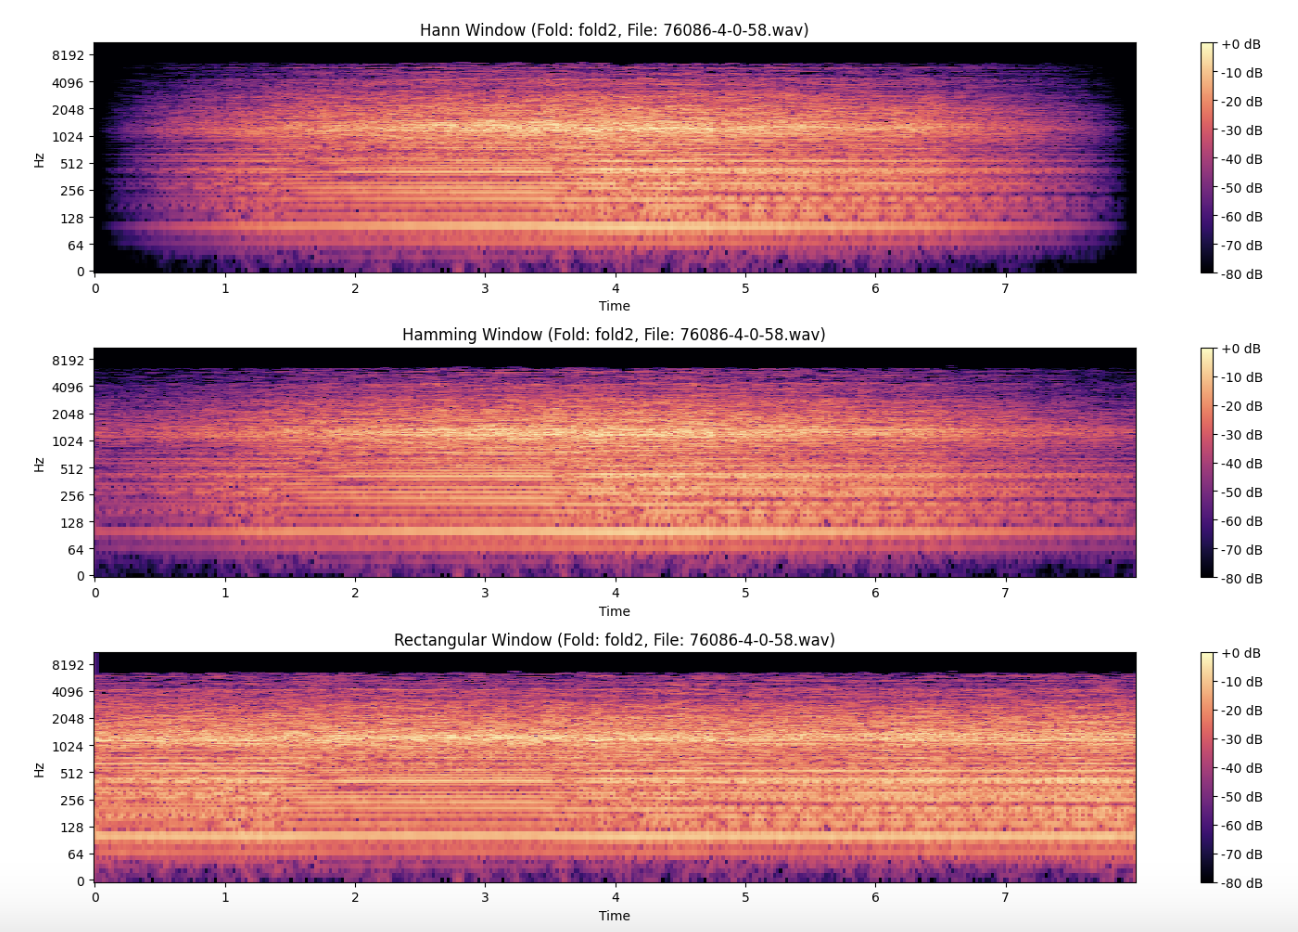
\includegraphics[width=1\linewidth]{Fold2.png}
    \end{figure}
    \begin{itemize}
        \item All spectrograms cover a frequency range from  \textbf{0 Hz to 8192 Hz}.
        \item Each spectrogram has a frequency resolution of approximately \textbf{8.28 Hz per pixel}.
        \item The total time duration in all spectrograms is \textbf{7.5 seconds}.
        \item Time resolution is \textbf{0.0033 seconds per pixel}, meaning fine time variations are captured.
        \item \textbf{Hann Window}: Smooth transitions, minimizes spectral leakage, reduces intensity slightly.
        \item \textbf{Hamming Window}: Similar to Hann but preserves more mid-frequency details.
        \item \textbf{Rectangular Window}: Strongest intensity but introduces more noise and spectral artifacts.
        \item For precise and clear analysis, \textbf{Hann or Hamming} is preferred over the \textbf{Rectangular} window.
        \item For a better trade-off between smoothness and detail, \textbf{Hann or Hamming} is preferred over \textbf{Rectangular}.
    \end{itemize}
\newpage
    \subsubsection{Fold 3 : Spectrogram}
    \begin{figure}[H]
        \centering
        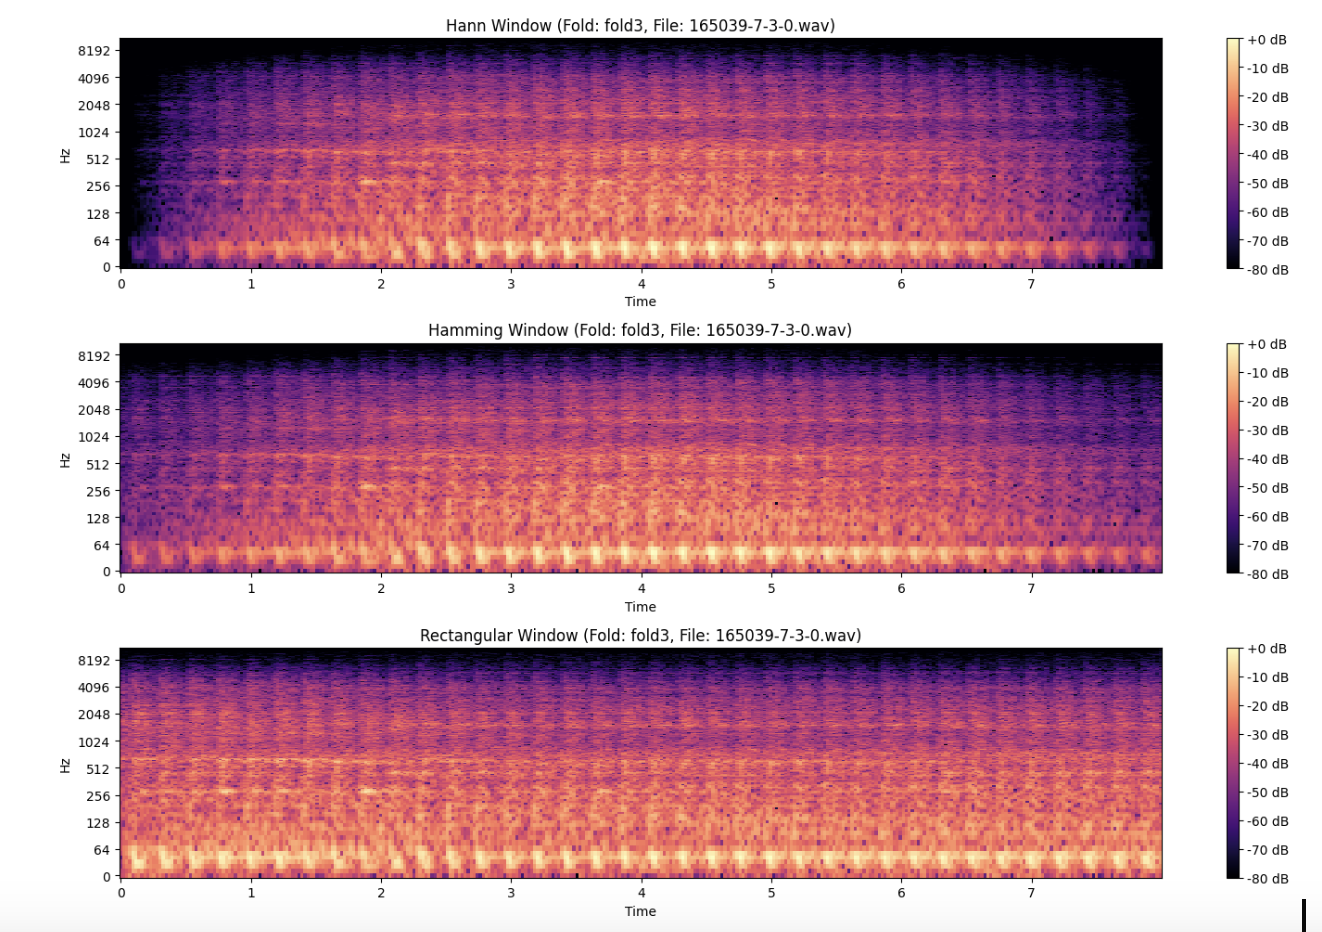
\includegraphics[width=1\linewidth]{Fold3.png}
    \end{figure}
    \begin{itemize}
        \item All spectrograms cover a frequency range from  \textbf{0 Hz to 8192 Hz}.
        \item Frequency resolution is \textbf{8.28 Hz per pixel}, ensuring fine frequency detail.
        \item The total time duration in all spectrograms is \textbf{7.5 seconds}.
        \item Time resolution is \textbf{0.0033 seconds per pixel}, which allows capturing rapid variations.
        \item \textbf{Hann Window}: Provides smooth transitions and minimizes spectral leakage, though it slightly reduces overall intensity.
        \item \textbf{Hamming Window}: Balances smoothness and detail retention, maintaining more mid-frequency information.
        \item \textbf{Rectangular Window}: Produces the highest intensity but introduces more spectral noise and artifacts.
        \item For optimal frequency analysis, \textbf{Hann or Hamming} is preferred over \textbf{Rectangular}.
    \end{itemize}
\newpage
    \subsubsection{Fold 4 : Spectrogram}
    \begin{figure}[H]
        \centering
        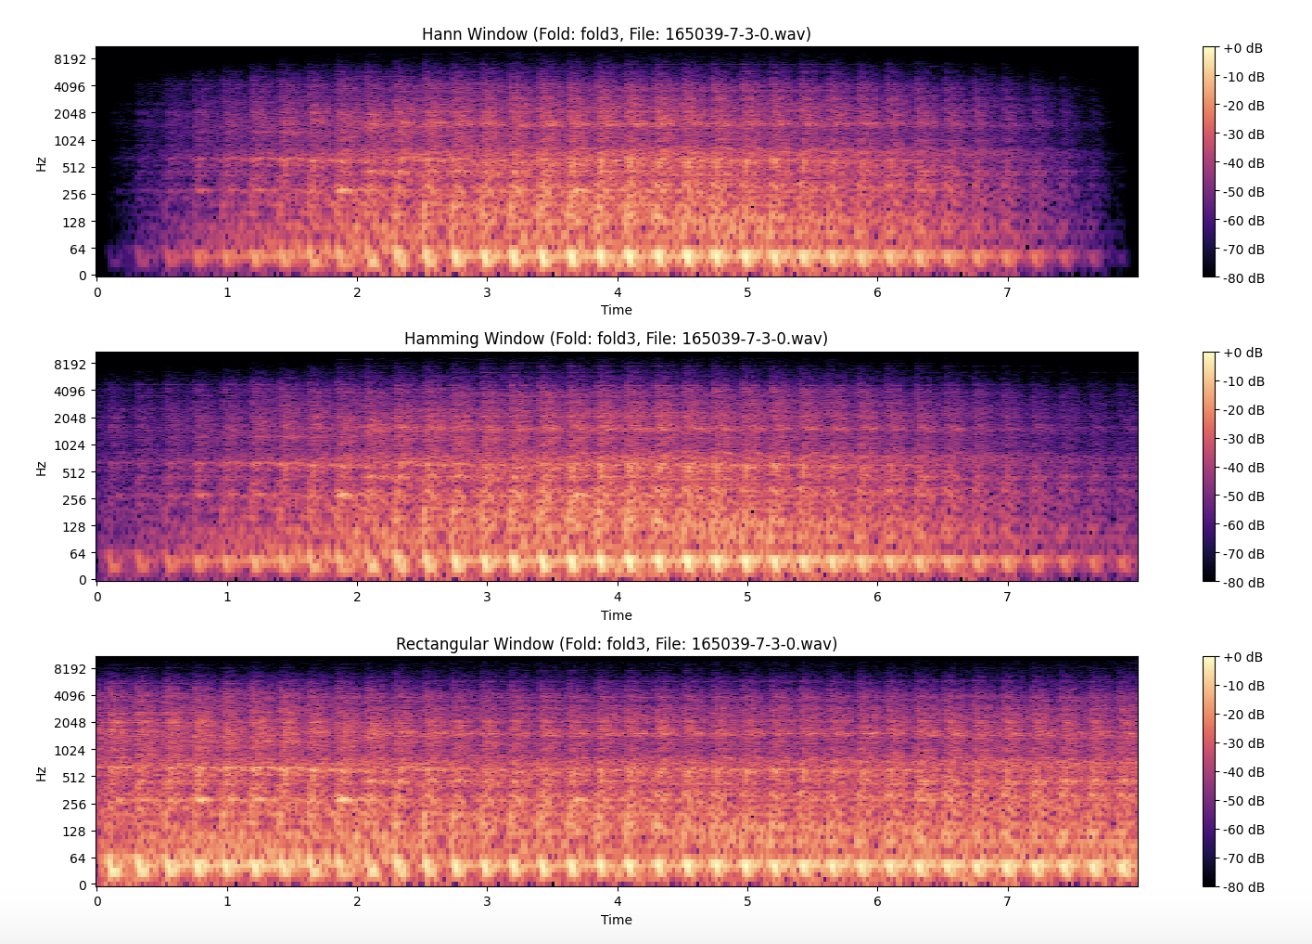
\includegraphics[width=1\linewidth]{Fold4.png}
    \end{figure}
    \begin{itemize}
        \item All spectrograms cover a frequency range from  \textbf{0 Hz to 8192 Hz}.
        \item Frequency resolution remains fine, allowing for detailed frequency analysis.
        \item The total time duration in all spectrograms is approximately \textbf{2.2 seconds}.
        \item Time resolution is high, capturing transient changes effectively.
        \item \textbf{Hann Window}: Smooth spectral transitions with minimized spectral leakage.
        \item \textbf{Hamming Window}: Slightly better intensity retention than Hann, while still reducing leakage.
        \item \textbf{Rectangular Window}: Produces the strongest intensity but introduces spectral artifacts and noise.
        \item The signal energy is concentrated in the \textbf{lower frequencies (below 1 kHz)}.
        \item Vertical patterns indicate periodic changes in amplitude.
        \item The \textbf{Rectangular Window} has the most visible noise, while \textbf{Hann and Hamming} provide cleaner representations.
    \end{itemize}
\newpage
    \subsubsection{Fold 5 : Spectrogram}
    \begin{figure}[H]
        \centering
        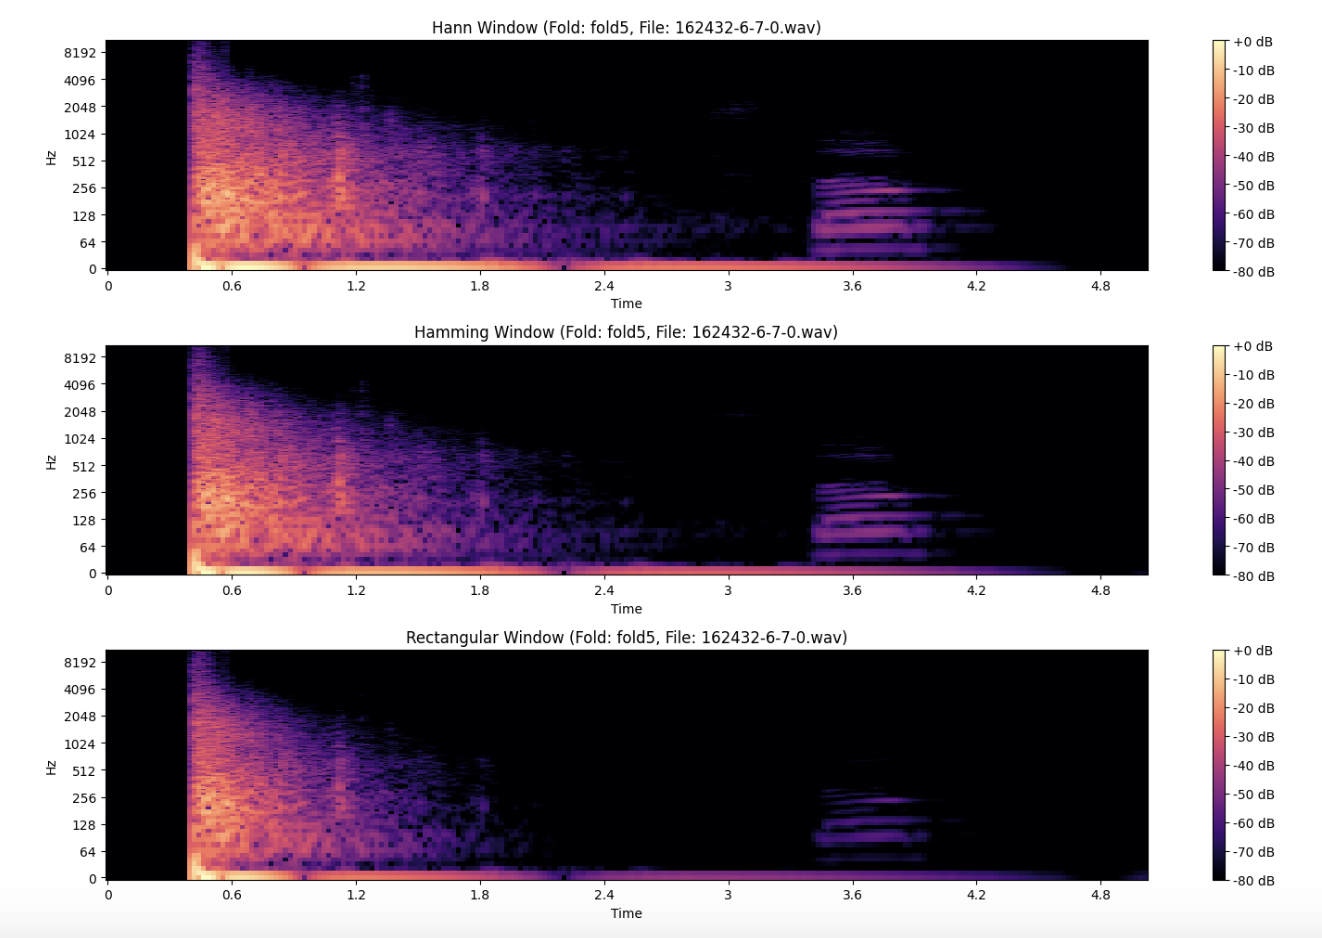
\includegraphics[width=1\linewidth]{Fold5.png}
    \end{figure}
    \begin{itemize}
        \item All spectrograms cover a frequency range from  \textbf{0 Hz to 8192 Hz}.
        \item They all show clear details in the frequency patterns.
        \item The total time duration of the signal is about \textbf{4.8 seconds}.
        \item The spectrograms capture quick changes in the sound over time.
        \item \textbf{Hann Window}:  Smooth changes in sound with less unwanted noise.
        \item \textbf{Hamming Window}:  Keeps sound details a bit better than Hann, with low noise.
        \item \textbf{Rectangular Window}: Shows the loudest sounds but adds more noise and unwanted patterns.
        \item Most of the sound energy is in the lower frequencies (below 1 kHz).
        \item Vertical lines show repeating changes in the sound.
        \item The Rectangular Window has the most noise, while Hann and Hamming show clearer sounds.
    \end{itemize}
\newpage
    \subsubsection{Fold 6 : Spectrogram}
    \begin{figure}[H]
        \centering
        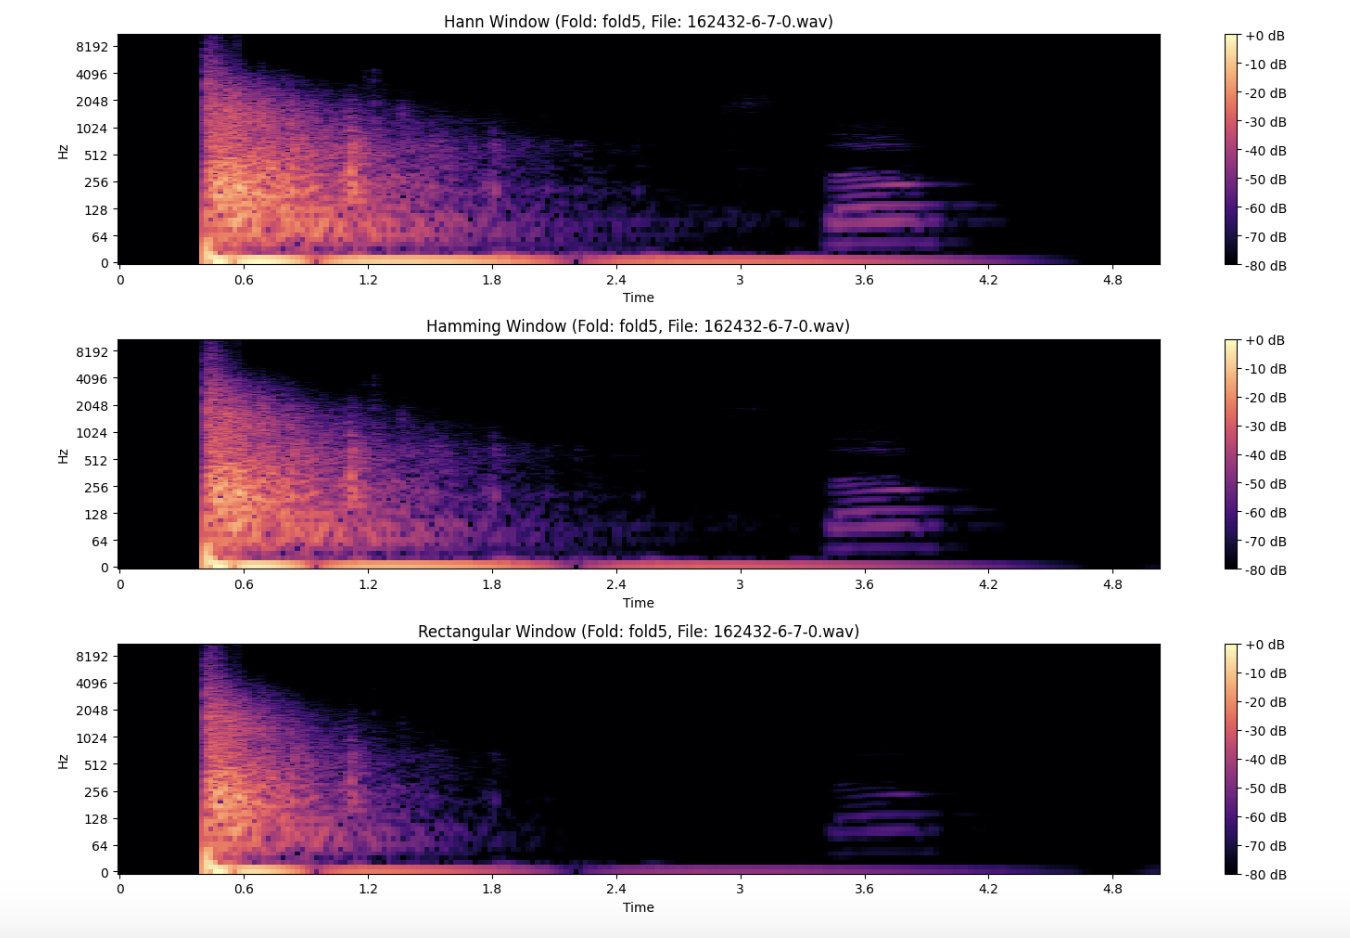
\includegraphics[width=1\linewidth]{Fold6.png}
    \end{figure}
    \begin{itemize}
        \item All spectrograms cover a frequency range from  \textbf{0 Hz to 8192 Hz}.
        \item They all show clear details in the frequency patterns.
        \item The total time duration of the signal is about \textbf{4.8 seconds}.
        \item The spectrograms capture quick changes in the sound over time.
        \item \textbf{Hann Window}:  Provides smooth spectral transitions with reduced background noise.
        \item \textbf{Hamming Window}: Offers a good balance between detail retention and noise suppression.
        \item \textbf{Rectangular Window}: Displays higher intensity but introduces more spectral leakage and noise.
    \end{itemize}
\newpage
    \subsubsection{Fold 7 : Spectrogram}
    \begin{figure}[H]
        \centering
        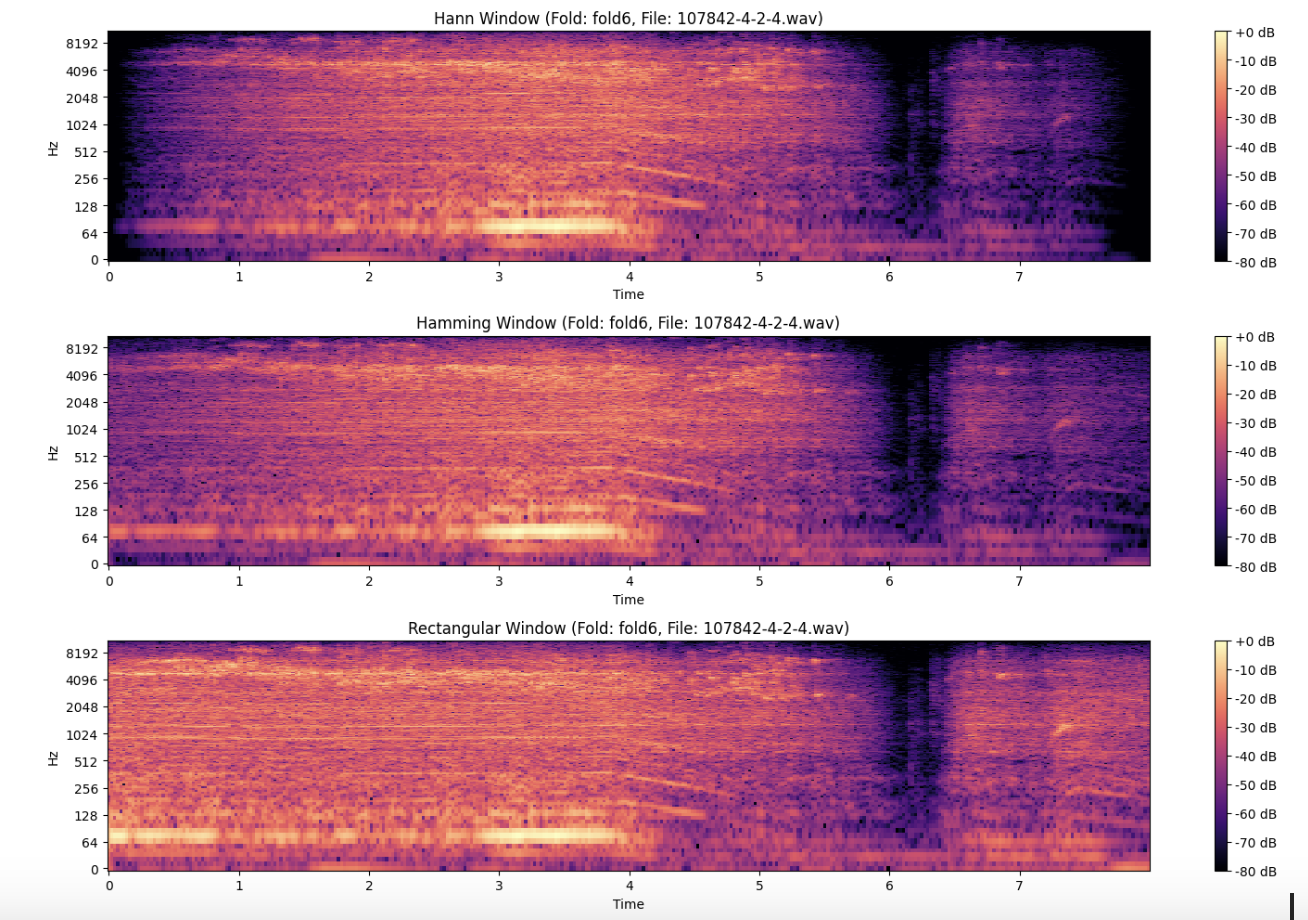
\includegraphics[width=1\linewidth]{Fold7.png}
    \end{figure}
    \begin{itemize}
        \item Also spans 0 Hz to 8192 Hz.
        \item Maintains detailed frequency patterns similar to Fold6.
        \item Covers approximately 4.8 seconds.
        \item Effectively captures transient changes in the audio signal.
        \item \textbf{Hann Window}:  Ensures smooth spectral representation with minimal noise artifacts.
        \item \textbf{Hamming Window}: Retains important sound details while keeping noise low.
        \item \textbf{Rectangular Window}: Emphasizes louder components but at the cost of increased noise and spectral leakage.
    \end{itemize}
\newpage
    \subsubsection{Fold 8 : Spectrogram}
    \begin{figure}[H]
        \centering
        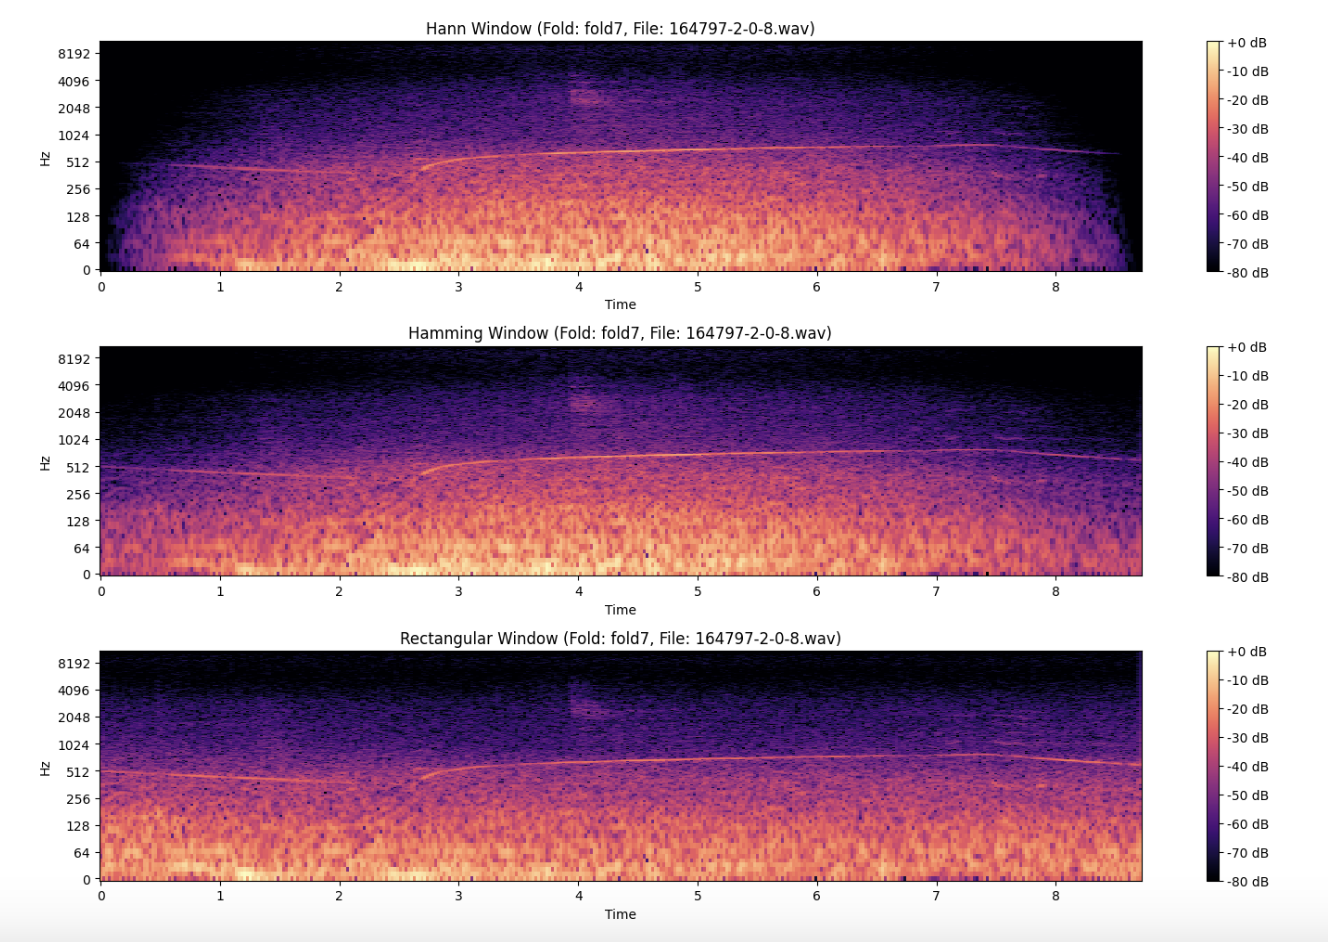
\includegraphics[width=1\linewidth]{Fold8.png}
    \end{figure}
    \begin{itemize}
        \item All spectrograms show frequencies from  \textbf{0 Hz to 8192 Hz}.
        \item The frequency details are clear in all three cases.
        \item The spectrograms cover a total time of about  \textbf{7 seconds}.
        \item They show changes over time clearly and with good detail.
        \item The signal energy is predominantly concentrated in the \textbf{lower frequency range (below 1 kHz)}, as indicated by the higher intensity in these regions.
        \item Vertical patterns in the spectrograms suggest periodic changes in the signal's amplitude or modulated frequencies.
        \item The \textbf{Rectangular Window} exhibits the most visible noise and artifacts, making it less suitable for accurate spectral analysis.
        \item \textbf{Hann Window}: delivers the cleanest output, followed by the \textbf{Hamming Window}.
        \item \textbf{Energy Focus}: Most of the energy is in lower frequencies, especially below \textbf{1 kHz}.
        \item \textbf{Patterns Over Time:} Vertical lines show periodic changes in the signal.
        \item \textbf{Noise:} The Rectangular Window has the most noise and artifacts, while the Hann and Hamming windows give cleaner results.
    \end{itemize}
\newpage
    \subsubsection{Fold 9 : Spectrogram}
    \begin{figure}[H]
        \centering
        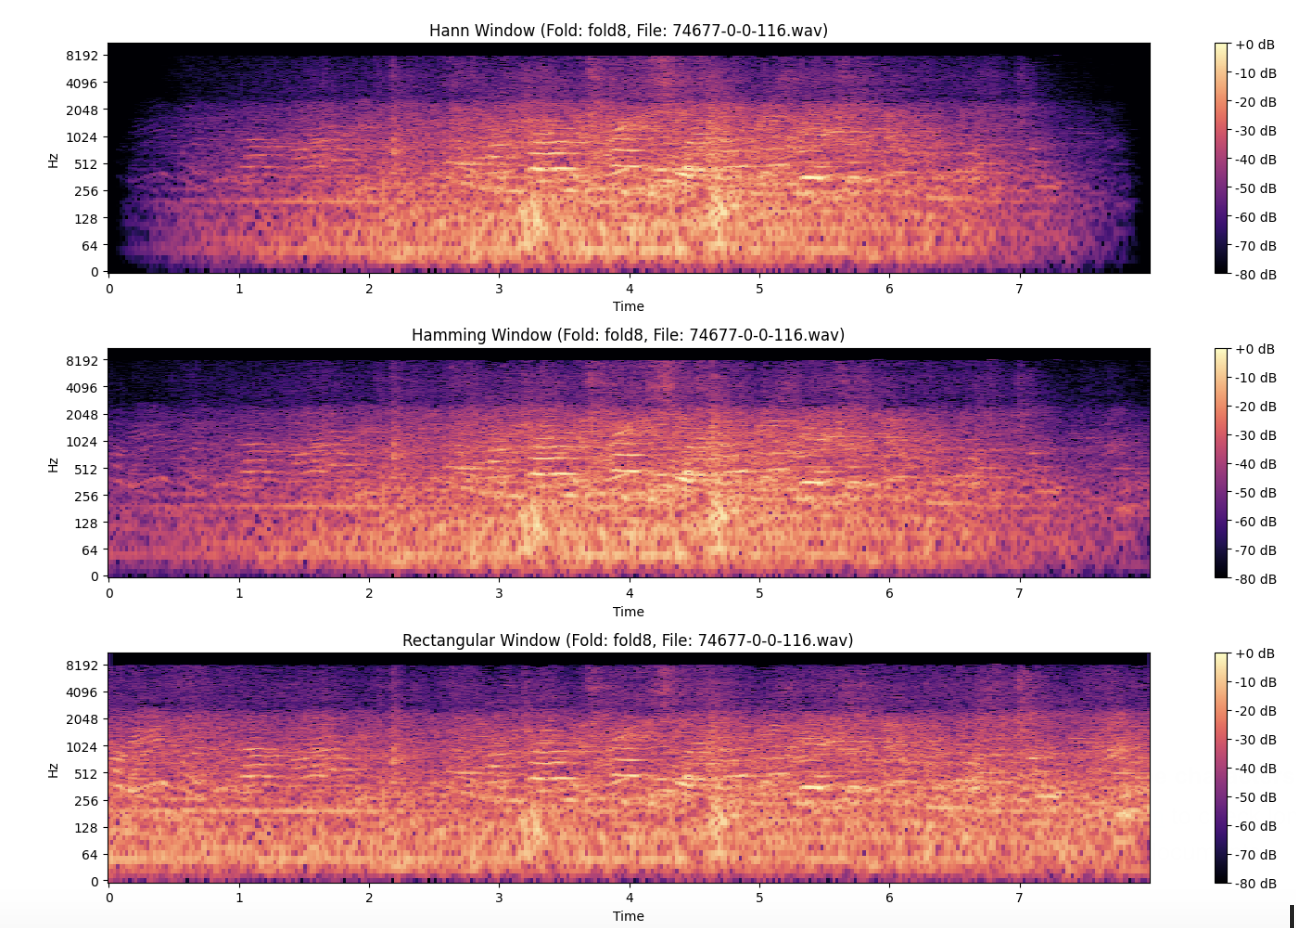
\includegraphics[width=1\linewidth]{Fold9.png}
    \end{figure}
    \begin{itemize}
        \item All spectrograms show frequencies from  \textbf{0 Hz to 8192 Hz}.
        \item Frequency details are well-resolved in all three cases, showing clear variations across the range.
        \item The total signal duration is approximately  \textbf{7 seconds}.
        \item The spectrograms capture the signal's time-dependent changes clearly.
        \item \textbf{Hann Window:} Best for reducing noise and ensuring a smooth representation of the signal.
        \item \textbf{Hamming Window:} Offers a balance between strong intensity and smoothness, making it a versatile option.
        \item \textbf{Hann Window:} Shows higher intensity but is less suitable for analysis due to more noise and artifacts.
        \item The \textbf{Rectangular Window:}
            \begin{itemize}
                \item Shows the strongest intensity of all three techniques.
                \item However, it introduces noticeable noise and artifacts, making the spectrogram less clean.
            \end{itemize}
        \item \textbf{Energy Focus:} Most of the energy is concentrated in lower frequencies, primarily below \textbf{1 kHz}, with some activity extending beyond.
        \item \textbf{Periodic Patterns:} Vertical variations in intensity indicate periodic changes in the signal's characteristics over time.
    \end{itemize}
\newpage
    \subsubsection{Fold 10 : Spectrogram}
    \begin{figure}[H]
        \centering
        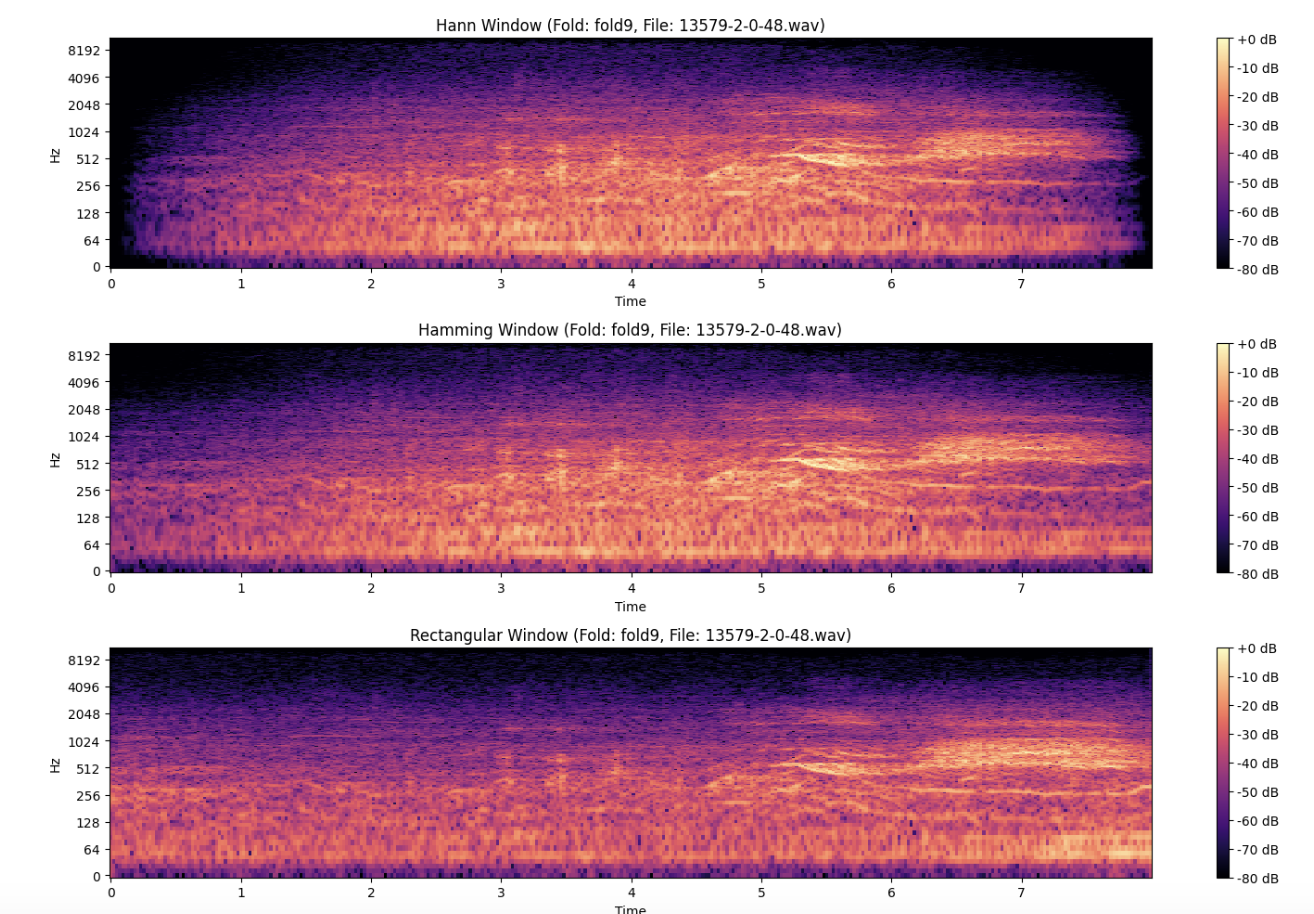
\includegraphics[width=1\linewidth]{Fold10.png}
    \end{figure}
    \begin{itemize}
        \item All spectrograms show frequencies from  \textbf{0 Hz to 8192 Hz}.
        \item Frequency details are clearly visible, showing good resolution.
        \item The signal duration spans approximately  \textbf{8 seconds}.
        \item The spectrograms capture changes over time effectively, allowing for clear time-frequency analysis.
        \item \textbf{Energy Focus:} The energy is concentrated in lower frequencies, particularly below \textbf{1 kHz}, with noticeable harmonic structures at higher frequencies.
        \item \textbf{Harmonic Patterns:} Horizontal lines in the spectrograms represent harmonics of the signal.
        \item \textbf{Noise Levels:}
            \begin{itemize}
                \item The \textbf{Rectangular Window} exhibits more noise and less-defined harmonic structures.
                \item The \textbf{Hann and Hamming Windows} produce cleaner and more defined spectrograms.
            \end{itemize}
        \item \textbf{Hann Window:} Best for smooth and noise-free spectral analysis.
        \item \textbf{Hamming Window:} A good compromise between smoothness and intensity, providing clear harmonics.
        \item \textbf{Rectangular Window:} Stronger intensity but less suitable due to increased noise and artifacts.
    \end{itemize}
\newpage
\section{Training a SVM Using Spectrogram Features}
We train a simple classifier (SVM) using features extracted from spectrograms of audio signals. The performance of the classifier is evaluated for different windowing techniques (Hann, Hamming, Rectangular), and the results are compared to determine the most effective technique.
    \subsection{Methodology}
        \subsubsection{Dataset:}
            \begin{itemize}
                \item The UrbanSound8K dataset is used, which contains audio files from 10 different classes 
                \item The dataset is divided into 10 folds, and a subset of the data is used for training and testing.
            \end{itemize}
        \subsubsection{Feature Extraction:}
            \begin{itemize}
                \item Spectrograms are generated using the Short-Time Fourier Transform (STFT) for each audio file.
                \item Three windowing techniques are applied: Hann, Hamming, and Rectangular windows.
                \item Features are extracted from the spectrograms by computing the mean and standard deviation of the frequency bins.
            \end{itemize}
        \subsubsection{Classifier:}
            \begin{itemize}
                \item A Support Vector Machine (SVM) with a linear kernel is used as the classifier.
                \item The dataset is split into training and testing sets (80% training, 20% testing).
                \item The classifier is trained and evaluated for each windowing technique.
            \end{itemize}
        \subsubsection{Evaluation Metrics:}
            \begin{itemize}
                \item Accuracy: Measures the percentage of correctly classified samples.
                \item Classification Report: Provides precision, recall, and F1-score for each class.
                \item Confusion Matrix: Visualizes the performance of the classifier for each class.
                \item Training Time: Measures the time taken to train the classifier.
            \end{itemize}
    \subsection{Results}
        \subsubsection{Performance Comparison of Windowing Techniques}
            \begin{figure}[H]
                \centering
                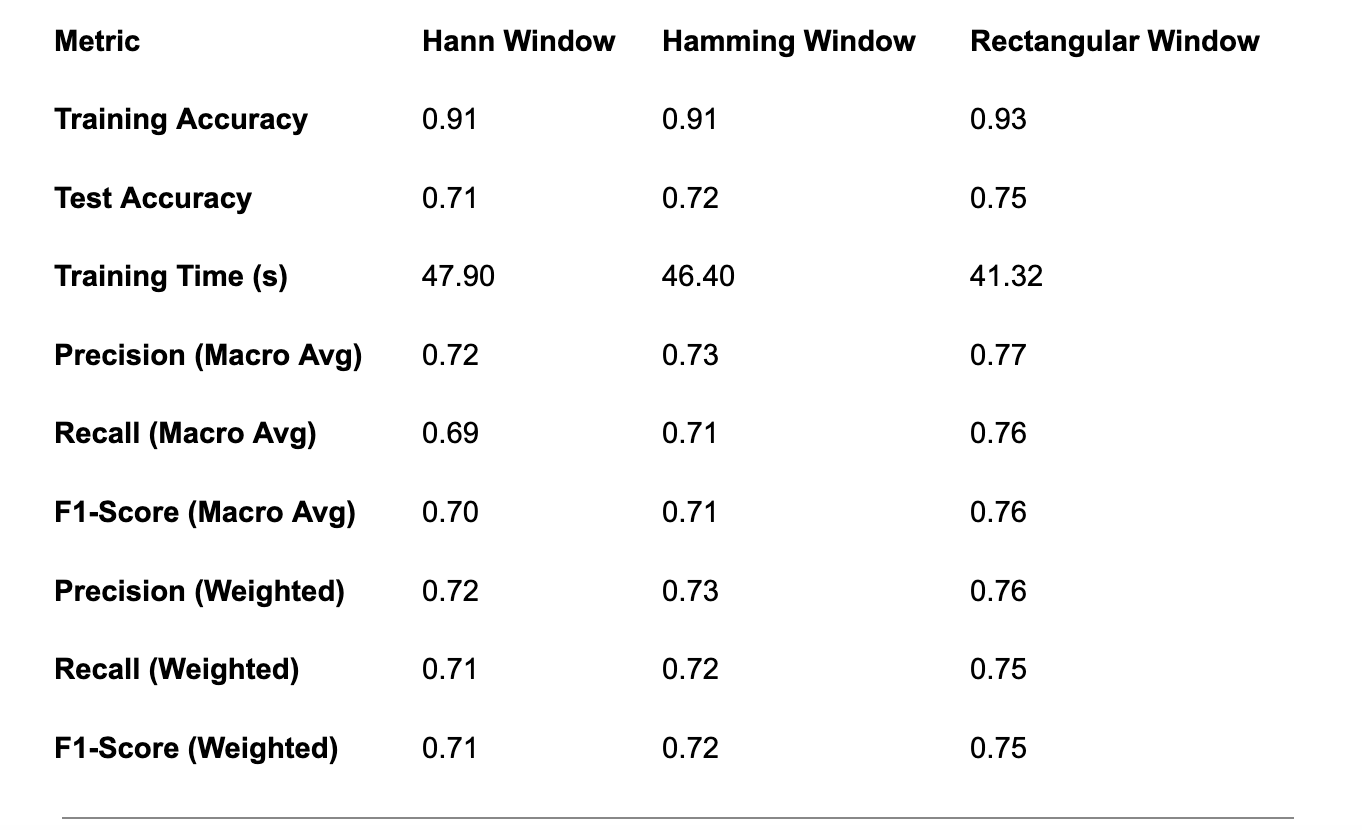
\includegraphics[width=1\linewidth]{PerformanceComparison.png}
            \end{figure}
            \begin{figure}[H]
                \centering
                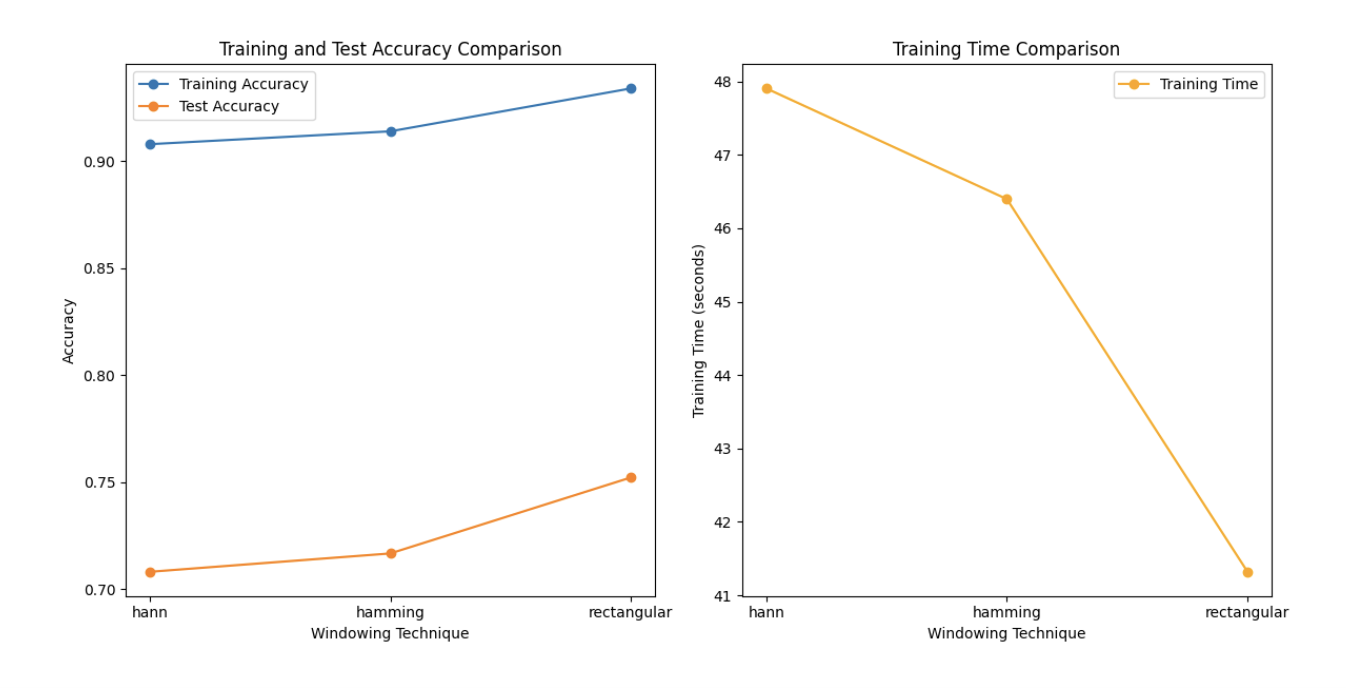
\includegraphics[width=1\linewidth]{PerformanceComparisonChart.png}
            \end{figure}
            \begin{figure}[H]
                \centering
                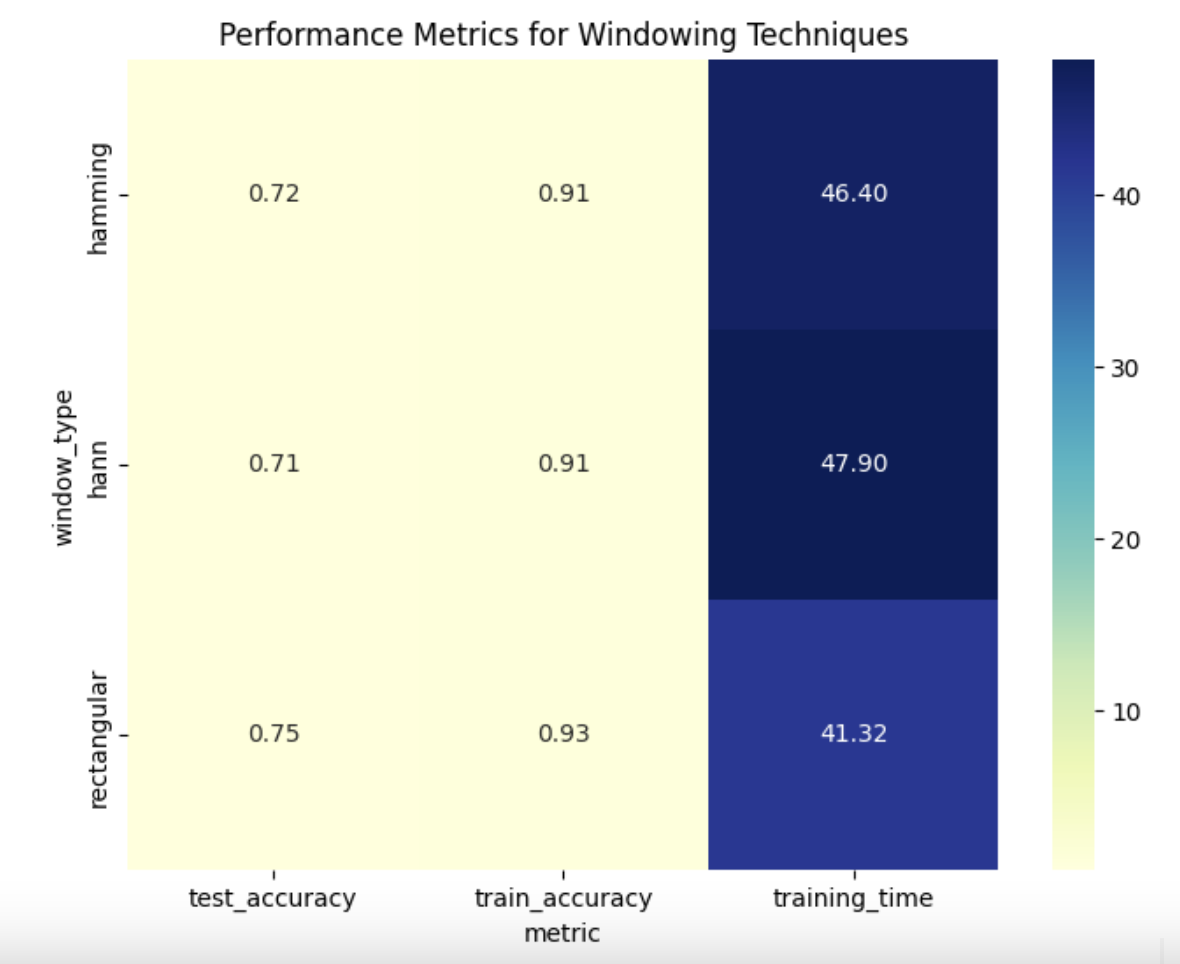
\includegraphics[width=1\linewidth]{PerformanceMetricsWindowing.png}
            \end{figure}
        \subsubsection{Key Observations from the Table}
            \begin{enumerate}
                \item Test Accuracy:
                    \begin{itemize}
                        \item Rectangular Window achieved the highest test accuracy (0.75), followed by Hamming Window (0.72) and Hann Window (0.71).
                    \end{itemize}
                \item Training Time:
                    \begin{itemize}
                        \item Rectangular Window was the fastest to train (41.32 seconds), while Hann Window took the longest (47.90 seconds).
                    \end{itemize}
                \item Precision, Recall, and F1-Score:
                    \begin{itemize}
                        \item The Rectangular Window consistently outperformed the other two techniques in terms of precision, recall, and F1-score (both macro and weighted averages).
                    \end{itemize}
                \item Overall Performance:
                    \begin{itemize}
                        \item The Rectangular Window provided the best balance between accuracy, training time, and classification performance.
                    \end{itemize}
                \item Confusion Matrix:
                    \begin{itemize}
                        \item The confusion matrices for all three windowing techniques showed that the classifier performed well for most classes but struggled with some ( class 3 and class 9).
                    \end{itemize}
            \end{enumerate}
\newpage
\subsection{Conclusion}
    \begin{itemize}
        \item The Rectangular window outperformed the Hann and Hamming windows in terms of test accuracy, training time, and classification performance.
        \item Despite its simplicity, the Rectangular window provided the best balance between accuracy and computational efficiency for this task.
        \item The Hamming window performed slightly better than the Hann window, but both were less effective than the Rectangular window.
    \end{itemize}
\newpage
\section{Code Repository} 
\href{https://github.com/IITJ-M23CSA521/M23CSA521_PA1.git}{GitHub Repository URL}
\addcontentsline{toc}{section}{References}
%\addbibresource{references.bib}
%\printbibliography[heading=bibintoc, title={References}]
\begin{thebibliography}{9}
    \bibitem{example} \href{https://www.geeksforgeeks.org/audio-classification-using-spectrograms/}{Audio classification using spectrograms}
    \bibitem{example2} \href{https://www.kaggle.com/code/prabhavsingh/urbansound8k-classification}{ UrbanSound8K - Classification}
    \bibitem{example3} \href{https://www.kaggle.com/code/adinishad/urbansound-classification-with-pytorch-and-fun}{ UrbanSound Classification with Pytorch and Fun}
     \bibitem{documentation} \href{https://www.overleaf.com/}{ Latex Documentation - Overleaf}
     \bibitem{windowing} \href{https://www.slideshare.net/slideshow/windowing-signal-processing/83279017}{Windowing (signal processing)}
     \bibitem{spectrograms} \href{https://www.izotope.com/en/learn/understanding-spectrograms.html}{Understanding spectrograms}
\end{thebibliography}

\end{document}
